\hypertarget{pf__administration_8c}{
\section{pf\_\-administration.c File Reference}
\label{pf__administration_8c}\index{pf\_\-administration.c@{pf\_\-administration.c}}
}
{\tt \#include $<$stdio.h$>$}\par
{\tt \#include $<$stdlib.h$>$}\par
{\tt \#include $<$errno.h$>$}\par
{\tt \#include $<$string.h$>$}\par
{\tt \#include $<$sqlite3.h$>$}\par
{\tt \#include \char`\"{}libphonefirewall.h\char`\"{}}\par


Include dependency graph for pf\_\-administration.c:\nopagebreak
\begin{figure}[H]
\begin{center}
\leavevmode
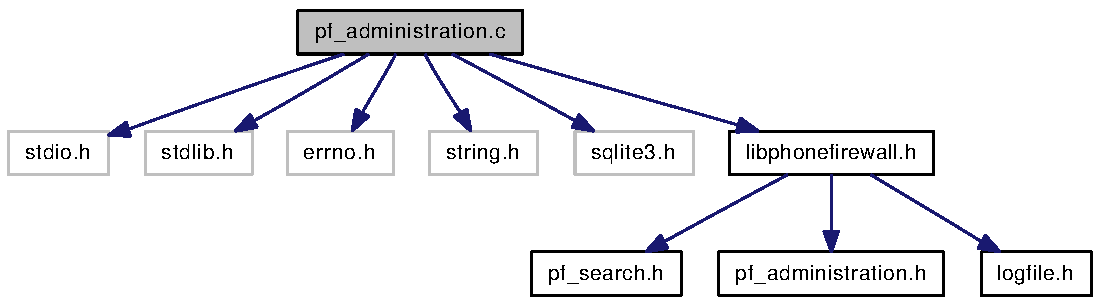
\includegraphics[width=281pt]{pf__administration_8c__incl}
\end{center}
\end{figure}
\subsection*{Functions}
\begin{CompactItemize}
\item 
int \hyperlink{pf__administration_8c_f306b60195d745190ef3e30e7d0a107e}{evaluate\_\-stmt} (sqlite3\_\-stmt $\ast$pp\_\-stmt, struct \hyperlink{structEntry}{Entry} $\ast$p\_\-entry)
\item 
int \hyperlink{pf__administration_8c_6c03680796f887d3851428fb2b9ecbc5}{add\_\-entry} (int country\_\-code, int area\_\-code, unsigned long long number, char $\ast$name, char $\ast$reason, int priority, int listflag)
\item 
int \hyperlink{pf__administration_8c_ab5a3f8ece1e8f7c4f11d003a10f7403}{rm\_\-entry} (int country\_\-code, int area\_\-code, unsigned long long number, int listflag)
\item 
int \hyperlink{pf__administration_8c_754e9a8891128a285fc17132b5480a07}{check\_\-entry} (int country\_\-code, int area\_\-code, unsigned long long number, int priority, int listflag)
\end{CompactItemize}


\subsection{Function Documentation}
\hypertarget{pf__administration_8c_6c03680796f887d3851428fb2b9ecbc5}{
\index{pf\_\-administration.c@{pf\_\-administration.c}!add\_\-entry@{add\_\-entry}}
\index{add\_\-entry@{add\_\-entry}!pf_administration.c@{pf\_\-administration.c}}
\subsubsection{\setlength{\rightskip}{0pt plus 5cm}int add\_\-entry (int {\em country\_\-code}, int {\em area\_\-code}, unsigned long long {\em number}, char $\ast$ {\em name}, char $\ast$ {\em reason}, int {\em priority}, int {\em listflag})}}
\label{pf__administration_8c_6c03680796f887d3851428fb2b9ecbc5}


Add a number to the blacklist/whitelist. The number will be blocked after that.

\begin{Desc}
\item[Parameters:]
\begin{description}
\item[{\em country\_\-code}]The country code (for example 39 for Italy, 43 for Austria, and so one) \item[{\em area\_\-code}]The area code which indicates your mobile operator. \item[{\em number}]The telephone number of the person (without country and area code. \item[{\em name}]The name of the person. \item[{\em reason}]Why you have blocked this person. \item[{\em priority}]Gives the \hyperlink{structentry}{entry} a priority. 0 is standard. If the priority is higher the value will be also blocked/accepted if a higher priority is choosen. \item[{\em listflag}]A flag, which indicates if you would use the blacklist (BLACKLIST\_\-FLAG) or the whitelist (WHITELIST\_\-FLAG).\par
\end{description}
\end{Desc}
The value \char`\"{}PRIO\_\-ALL\char`\"{} stands for all priorities.

\begin{Desc}
\item[Returns:]If all goes well 0 (zero) otherwise -1 and the errno variable will be set.. \end{Desc}


Definition at line 74 of file pf\_\-administration.c.

References BLACKLIST\_\-FLAG, DB\_\-FILE, ERR\_\-LOG, MAX\_\-LINE\_\-LENGTH, PRIO\_\-ALL, STMT\_\-SIZE, TB\_\-AREACODE, TB\_\-COUNTRYCODE, TB\_\-NAME, TB\_\-NUMBER, TB\_\-PRIORITY, TB\_\-REASON, and WHITELIST\_\-FLAG.\hypertarget{pf__administration_8c_754e9a8891128a285fc17132b5480a07}{
\index{pf\_\-administration.c@{pf\_\-administration.c}!check\_\-entry@{check\_\-entry}}
\index{check\_\-entry@{check\_\-entry}!pf_administration.c@{pf\_\-administration.c}}
\subsubsection{\setlength{\rightskip}{0pt plus 5cm}int check\_\-entry (int {\em country\_\-code}, int {\em area\_\-code}, unsigned long long {\em number}, int {\em priority}, int {\em listflag})}}
\label{pf__administration_8c_754e9a8891128a285fc17132b5480a07}


Checks if a number is on the blacklist/whitelist.

\begin{Desc}
\item[Parameters:]
\begin{description}
\item[{\em country\_\-code}]The country code (for example 39 for Italy, 43 for Austria, and so one) \item[{\em area\_\-code}]The area code which indicates your mobile operator. \item[{\em number}]The telephone number of the person (without country and area code. \item[{\em priority}]Gives the \hyperlink{structentry}{entry} a priority. 0 is standard. If the priority is higher the value will be also blocked/accepted if a higher priority is choosen. \item[{\em listflag}]A flag, which indicates if you would use the blacklist (BLACKLIST\_\-FLAG) or the whitelist (WHITELIST\_\-FLAG).\par
\end{description}
\end{Desc}
The value \char`\"{}PRIO\_\-ALL\char`\"{} stands for all priorities.

\begin{Desc}
\item[Returns:]If the number was found 1, otherwise 0. \end{Desc}


Definition at line 174 of file pf\_\-administration.c.

References Entry::area\_\-code, BLACKLIST\_\-FLAG, Entry::country\_\-code, DB\_\-FILE, ERR\_\-LOG, evaluate\_\-stmt(), INFO\_\-LOG, MAX\_\-LINE\_\-LENGTH, Entry::number, Entry::priority, STMT\_\-SIZE, TB\_\-AREACODE, TB\_\-COUNTRYCODE, TB\_\-NUMBER, TB\_\-PRIORITY, and WHITELIST\_\-FLAG.

Here is the call graph for this function:\nopagebreak
\begin{figure}[H]
\begin{center}
\leavevmode
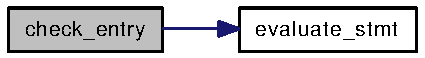
\includegraphics[width=120pt]{pf__administration_8c_754e9a8891128a285fc17132b5480a07_cgraph}
\end{center}
\end{figure}
\hypertarget{pf__administration_8c_f306b60195d745190ef3e30e7d0a107e}{
\index{pf\_\-administration.c@{pf\_\-administration.c}!evaluate\_\-stmt@{evaluate\_\-stmt}}
\index{evaluate\_\-stmt@{evaluate\_\-stmt}!pf_administration.c@{pf\_\-administration.c}}
\subsubsection{\setlength{\rightskip}{0pt plus 5cm}int evaluate\_\-stmt (sqlite3\_\-stmt $\ast$ {\em pp\_\-stmt}, struct {\bf Entry} $\ast$ {\em p\_\-entry})}}
\label{pf__administration_8c_f306b60195d745190ef3e30e7d0a107e}




Definition at line 27 of file pf\_\-administration.c.

References Entry::area\_\-code, Entry::country\_\-code, Entry::number, PRIO\_\-ALL, Entry::priority, TB\_\-AREACODE, TB\_\-COUNTRYCODE, TB\_\-NUMBER, and TB\_\-PRIORITY.

Referenced by check\_\-entry().

Here is the caller graph for this function:\nopagebreak
\begin{figure}[H]
\begin{center}
\leavevmode
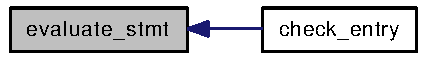
\includegraphics[width=120pt]{pf__administration_8c_f306b60195d745190ef3e30e7d0a107e_icgraph}
\end{center}
\end{figure}
\hypertarget{pf__administration_8c_ab5a3f8ece1e8f7c4f11d003a10f7403}{
\index{pf\_\-administration.c@{pf\_\-administration.c}!rm\_\-entry@{rm\_\-entry}}
\index{rm\_\-entry@{rm\_\-entry}!pf_administration.c@{pf\_\-administration.c}}
\subsubsection{\setlength{\rightskip}{0pt plus 5cm}int rm\_\-entry (int {\em country\_\-code}, int {\em area\_\-code}, unsigned long long {\em number}, int {\em listlfag})}}
\label{pf__administration_8c_ab5a3f8ece1e8f7c4f11d003a10f7403}


Removes a number from the blacklist/whitelist.

\begin{Desc}
\item[Parameters:]
\begin{description}
\item[{\em country\_\-code}]The country code (for example 39 for Italy, 43 for Austria, and so one) \item[{\em area\_\-code}]The area code which indicates your mobile operator. \item[{\em number}]The number which will be deleted. \item[{\em listflag}]A flag, which indicates if you would use the blacklist (BLACKLIST\_\-FLAG) or the whitelist (WHITELIST\_\-FLAG).\par
\end{description}
\end{Desc}
\begin{Desc}
\item[Returns:]If all goes right 0, otherwise an error code. \end{Desc}


Definition at line 128 of file pf\_\-administration.c.

References BLACKLIST\_\-FLAG, DB\_\-FILE, ERR\_\-LOG, MAX\_\-LINE\_\-LENGTH, STMT\_\-SIZE, TB\_\-AREACODE, TB\_\-COUNTRYCODE, TB\_\-NUMBER, and WHITELIST\_\-FLAG.